\chapter{Gestión} \label{gestion}
Este capítulo engloba aquellos aspectos que tienen que ver diréctamente con la gestión del proyecto: la metodología que se ha seguido a lo largo de todo su desarrollo, la  recogida de los esfuerzos y la organización del trabajo así como el control de versiones de los diferentes componentes del proyecto. Se reserva un apartado para mencionar las diferentes pautas e imposiciones que han afectado a un desarrollo libre del proyecto y  se recoge un estudio acerca de la estimación del coste del proyecto en sí. 

\section{Metodología} \label{gestion.metodologia}
Este apartado explica la metodología que se ha seguido para llevar a cabo el desarrollo del proyecto, desde su fase inicial llamada prueba de concepto (Sección \ref{implementacion.prueba}) hasta su finalización. Se podrían distinguir dos fases conceptuales acordes a los diferentes \textit{modus operandi} del desarrollo: 
\paragraph*{Prueba de concepto.} El desarrollo de la prueba de concepto ha sido guiado por el director del proyecto. Esto es, el director del proyecto marcó inicialmente el panorama global y el diseño que se quería seguir. A partir de alli, el trabajo del alumno fue instalar y configurar las herramientas propuestas por el director y validar su integración mediante un flujo de datos de prueba. Si tras un período de pruebas exhaustivas algún componente fallaba o no cumplía con los requisitos especificados en el análisis del proyecto, dicho componente era desechado y se buscaba una alternativa viable al mismo. Lo mismo ocurría si alguna conexión de integración concreta fallaba; por ejemplo, en el caso de intentar conectar \textit{Hive} con \textit{JHipster} diréctamente, al comprobar que era una solución inviable que no cumplía con los requisitos del proyecto se decidió que la alternativa sería mantener la base de datos original de \textit{JHipster} (\textit{MySQL}) y agregar un componente intermedio (\textit{Sqoop}) para la transferencia de los datos desde \textit{Hive} a \textit{MySQL}.
\paragraph*{Prototipo.} Una vez integradas las diferentes herramientas y elegido el \textit{stack tecnológico} final, la implementación del prototipo real se ha llevado a cabo mediante una metodología iterativa. Teniendo en mente que se trata de un proyecto con un potencial de crecimiento casi ilimitado, la aproximación más lógica fue agregar valor al proyecto mediante una aproximación de iteraciones agregativas, empezando por la integración de los productos fitosanitarios autorizados de España y siguiendo por los datos acerca sustancias activas de la base de datos Europea sobre pesticidas.  Así pues, en la primera iteración se diseñó e implementó el flujo capaz de descargar los datos acerca de los productos fitosanitarios autorizados de España de la fuente, almacenarlos en \textit{Hadoop}, transformarlos y prepararlos para su inserción en \textit{Hive}, su transferencia a \textit{MySQL} y su posterior visualización en \textit{JHipster}. En una segunda iteración se realizó lo mismo pero con los datos de las sustancias activas extraídos de la base de datos Europea de pesticidas. Siguiendo esta metodología y con el objetivo fijado en el crecimiento del proyecto se puede observar que los futuros avances del sistema se pueden realizar de la misma manera. Otro desarrollador podría retomar el trabajo en este punto y hacer que el programa siga creciendo mediante la expansión del número de iteraciones que agreguen nuevos flujos de datos para dar sporte a nuevas fuentes. La tercera iteración supuso la agregación del soporte capaz de mapear los datos de la primera iteración con los de la segunda, en una versión más que nada ilustrativa; a pesar de que dicha integración no es capaz de mapear el 100\% de los datos, esto no es un problema peusto que no era el objetivo perseguido. Lo que se perseguía era validar el modelo de integración y dar soporte a un crecimiento sencillo de la solución. Por último, siguiendo esta filosofía de iteraciones se agregó en una cuarta iteración un mecanismo para la detección de errores o inconsistencias en los datos integrados provenientes de diferentes fuentes. 

\section{Organización y control de versiones} \label{gestion.organizacion}
Otro área de la gestión del proyecto es su organización, a través de sus diferentes componentes. En este apartado se pretende dar una visión global de las estructuras y tecnologías involucradas en la organización del proyecto. 
\par En primer lugar, cabe mencionar que las diferentes herramientas que constituyen el \textit{core }tecnológico del proyecto (\textit{Hadoop}, \textit{Hive}, \textit{Sqoop}, \textit{JHipster}, \textit{Talend}, \textit{MySQL}) se han instalado sobre el equipo del alumno, en una partición local del disco duro. Esto proporcionó rapidez de despliegue y desarrollo para el alumno pero podría suponer dificultades a la hora de expandir el proyecto e incluso riesgos adicionales debido a una inexistencia de tolerancia a fallos o copias de seguridad. No obstante, tratándose de un \textit{TFG} se asumieron los riesgos y se adoptó esta postura como la más adecuada. 
\par En segundo lugar, la propia gestión de las tareas a desarrollar durante el proyecto se ha controlado mediante \textit{Trello}\footnote{Trello - \url{https://trello.com}} a través de un \textit{\gls{kanban}} de cuatro columnas (\textit{To do}, \textit{Doing}, \textit{Problem} y \textit{Done}): 
\begin{itemize}
\item La columna \textit{To do} almacena aquellas tareas que están pendientes de realizar o figuran como \textit{features} posibles a desarrollar.
\item La columna \textit{Doing} contiene aquellas tareas que el alumno desarrollaba en cada momento.
\item La columna \textit{Problem} sirve para almacenar aquellas tareas que presentan algún problema y dificultan su terminación. A través del mecanismo de comentarios de \textit{Trello} el alumno dejaba redactado el problema que ha tenido en dicha tarea para tener constancia de ello en todo momento y posteriormente poder arreglarlo. 
\item La columna \textit{Done} es donde se arrastraban todas las tareas que eran terminadas.
\end{itemize} 
En la figura \ref{fig:trello} se puede observar el tablero que el alumno ha usado a lo largo de casi toda la duración del proyecto.

\begin{figure}[!b]
    \centering
    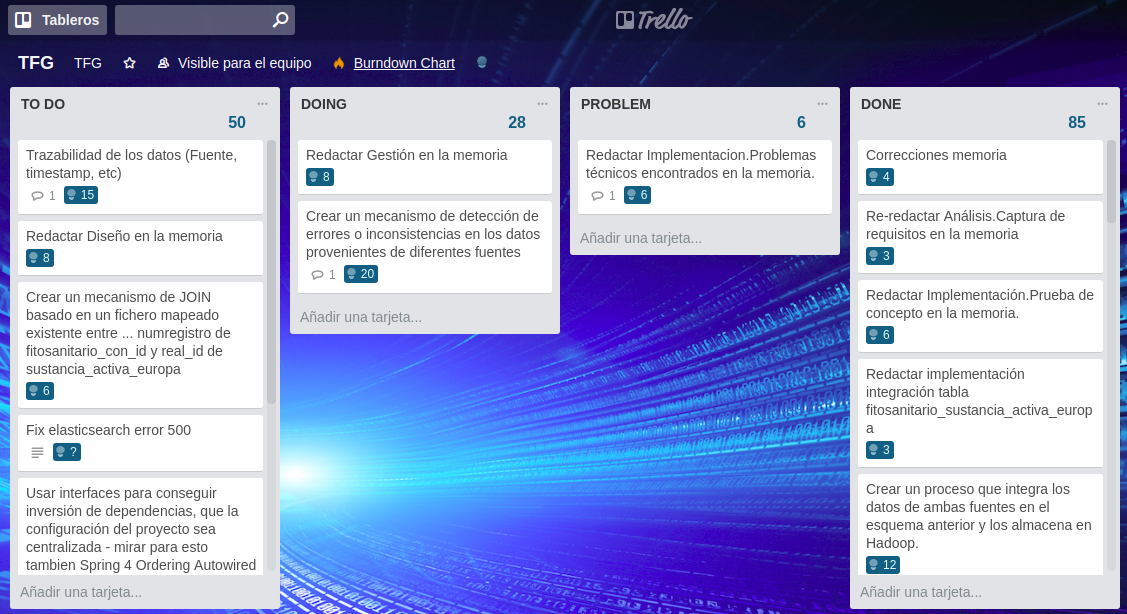
\includegraphics[width=\textwidth,height=\textheight,keepaspectratio]{Imagenes/trello}
    \caption{Tablero \textit{Trello} para la gestión de las tareas del proyecto.}
    \label{fig:trello}
\end{figure}

\par Otro aspecto de la organización se centra en la aplicación desarrollada con \textit{JHipster}. Inicialmente, esta se instaló al igual que las herramientas anteriores en el equipo local del alumno. No obstante, dado que sería una pieza fundamental y sobre la que se desarrollaría el software en sí, se decidió subirla a \textit{GIT} para mantener un control de versiones sobre ella. Profundizando más acerca de la organización del software desarrollado, dentro de la aplicación de \textit{JHipster} se creó un paquete encargado de mantener todo el código desarrollado por el alumno. Este paquete, llamado \textit{processes}, junto con sus subpaquetes y clases se puede observar en la figura \ref{fig:diag_clases}. Existe una clase principal llamada \textit{Schedule} encargada de lanzar los diferentes procesos. Aparte, se han designado distintos subpaquetes en función de las herramientas contra las que atacan: el paquete \textit{talend} es el que contiene los métodos encargados de ejecutar los trabajos desarrollados con \textit{Talend}. El paquete \textit{sqoop} contiene los métodos necesarios para poner en marcha una transferencia de \textit{Sqoop} desde \textit{Hive} a \textit{MySQL}. El paquete \textit{hive} contiene métodos que atacan contra la base de datos de \textit{Hive} mientras que el paquete \textit{mysql} contiene métodos que atacan contra la base de datos de \textit{MySQL}. El paquete \textit{common\_methods} es el único especial y contiene métodos públicos que puedan ser usados desde cualquiera de los demás paquetes. 
\par Como esta memoria también se quería mantener bajo un control de versiones riguroso, también se decidió que debería formar parte del software subido a \textit{GIT}. Así pues, en la carpeta raíz del proyecto de \textit{JHipster} se creó una carpeta llamada \textit{MEMORIA} donde se almacenaba todo lo referente a esta memoria.
\par Por último lugar, lo único restante de los diferentes componentes del proyecto son los diagramas desarrollados por el alumno tanto para el diseño de la aplicación como para los diferentes capítulos de la memoria y las hojas de gestión de esfuerzos. Estos componentes se crearon en \textit{Google Drive} y se han ido actualizando allí mismo. Dado que el alumno usa la aplicación web \textit{draw.io} propietaria de \textit{Google Drive} para realizar los diagramas, esta aproximación se consideró como la más adecuada. 

\section{Control de esfuerzos} \label{gestion.esfuerzos}

En la primera fase del proyecto el alumno desconocía el panorama global del desarrollo del \textit{TFG}; desconocía el hecho de que habría dos fases, una en la que se realizaría una prueba de concepto y otra en la que se desarrollaría un prototipo real a partir de la validación de las herramientas empleadas en esa prueba de concepto; teniendo esto en mente, cabe destacar que el alumno consideró que el primer contacto con las herramientas, es decir, su instalación y configuración formarían parte de una fase previa, una especie de requisitos previos al arranque del proyecto, que no contabilizarían como esfuerzos en sí. Es por ello que al principio del proyecto el alumno no tomó nota de las horas precisas invertidas en aquella primera fase que más tarde se le revelaría que formaría parte de la prueba de concepto. No obstante, gracias a las herramientas como \textit{Drive} o \textit{Trello}, posteriormente se pudo hacer una recopilación aproximada de los esfuerzos invertidos durante esta fase. Así pues, una vez que se determinó la estructura final del proyecto se empezó a tener constancia de las horas a través de una hoja de cálculo almacenada en \textit{Drive} y gracias a ello se pueden presentar los esfuerzos divididos en las siguientes categorías: 
\begin{itemize}
\item \textbf{Investigación. } El apartado de investigación incluye los diferentes esfuerzos realizados por el alumno para comprender la problemática actual que se intenta resolver en este \textit{TFG}, desde lecturas de manuales fitosanitarios hasta portales web que explican los procesos actuales de importación y exportación de los mismos. Se han dedicado aproximadamente 10 horas a este bloque.
\item \textbf{Análisis. } La fase de análisis comprendió un máximo de 20 horas aproximadas, entre la determinación de los requisitos, el análisis de los riesgos y la propia elección del \textit{Stack Tecnológico}. Aunque este último va diréctamente asociado a la prueba de concepto, cabe mencionarlo durante esta fase puesto que es donde a priori se analizaban las diferentes herramientas posibles de todo el elenco disponible. 
\item \textbf{Diseño. } El diseño del sistema tomó un máximo de 10 horas entre las diferentes variantes conceptuales; conforme se demostraba que un diseño aparente no cumplía con los requisitos del sistema, se procedía a diseñar otro, mejor adaptado a las necesidades del proyecto. 
\item \textbf{Prueba de concepto. } Al igual que las fases anteriores, gran parte de esta se ha desarrollado cuando aún no se tenía constancia precisa de las horas invertidas. No obstante, se pueden deducir alrededor de 80 horas totales que incluyen la instalación y configuración de las diferentes herramientas probadas junto con sus alternativas, las diferentes pruebas realizadas para conseguir un flujo de los datos desde su descarga hasta su transformación y presentación y la solventación de los diferentes errores que iban apareciéndo por el camino. 
\item \textbf{Implementación del prototipo real. } La implementación del prototipo real reune todos sus esfuerzos en la hoja de cálculo de \textit{Drive}, con un total de 63.5 \textbf{CAMBIAR SI NECESARIO} horas de dedicación. En ellas están incluidos los diferentes procesos desarrollados en \textit{Talend}, los diferentes mecanismos para su integración en \textit{Java}, los \textit{crawlers} implementados en lenguaje \textit{bash} así como los  componentes software desarrollados en \textit{Java}. 
\item \textbf{Reuniones con el director del proyecto. } Se pueden deducir unas 18 horas de reuniones con el director del proyecto aunque este apartado se puede entender como algo más flexible que los anteriores, ya que, si bien es cierto que no han habido muchas reuniones planificadas con el profesor, este iba pasando por el laboratorio en el que el alumno desarrollaba el trabajo para revisar con él los avances conseguidos y apoyarle en la consecución de los objetivos. 
\item \textbf{Redacción de la memoria. } Las horas invertidas en la redacción de la memoria, al igual que en el bloque anterior, se recogen en su totalidad en la hoja de cálculo de \textit{Drive}. Han resultado un total de 120.5 \textbf{CAMBIAR} horas.
\end{itemize}

En la figura \ref{fig:esfuerzos} se pueden observar las cifras anteriores en formato de diagrama de tarta. 

\begin{figure}[!h]
    \centering
    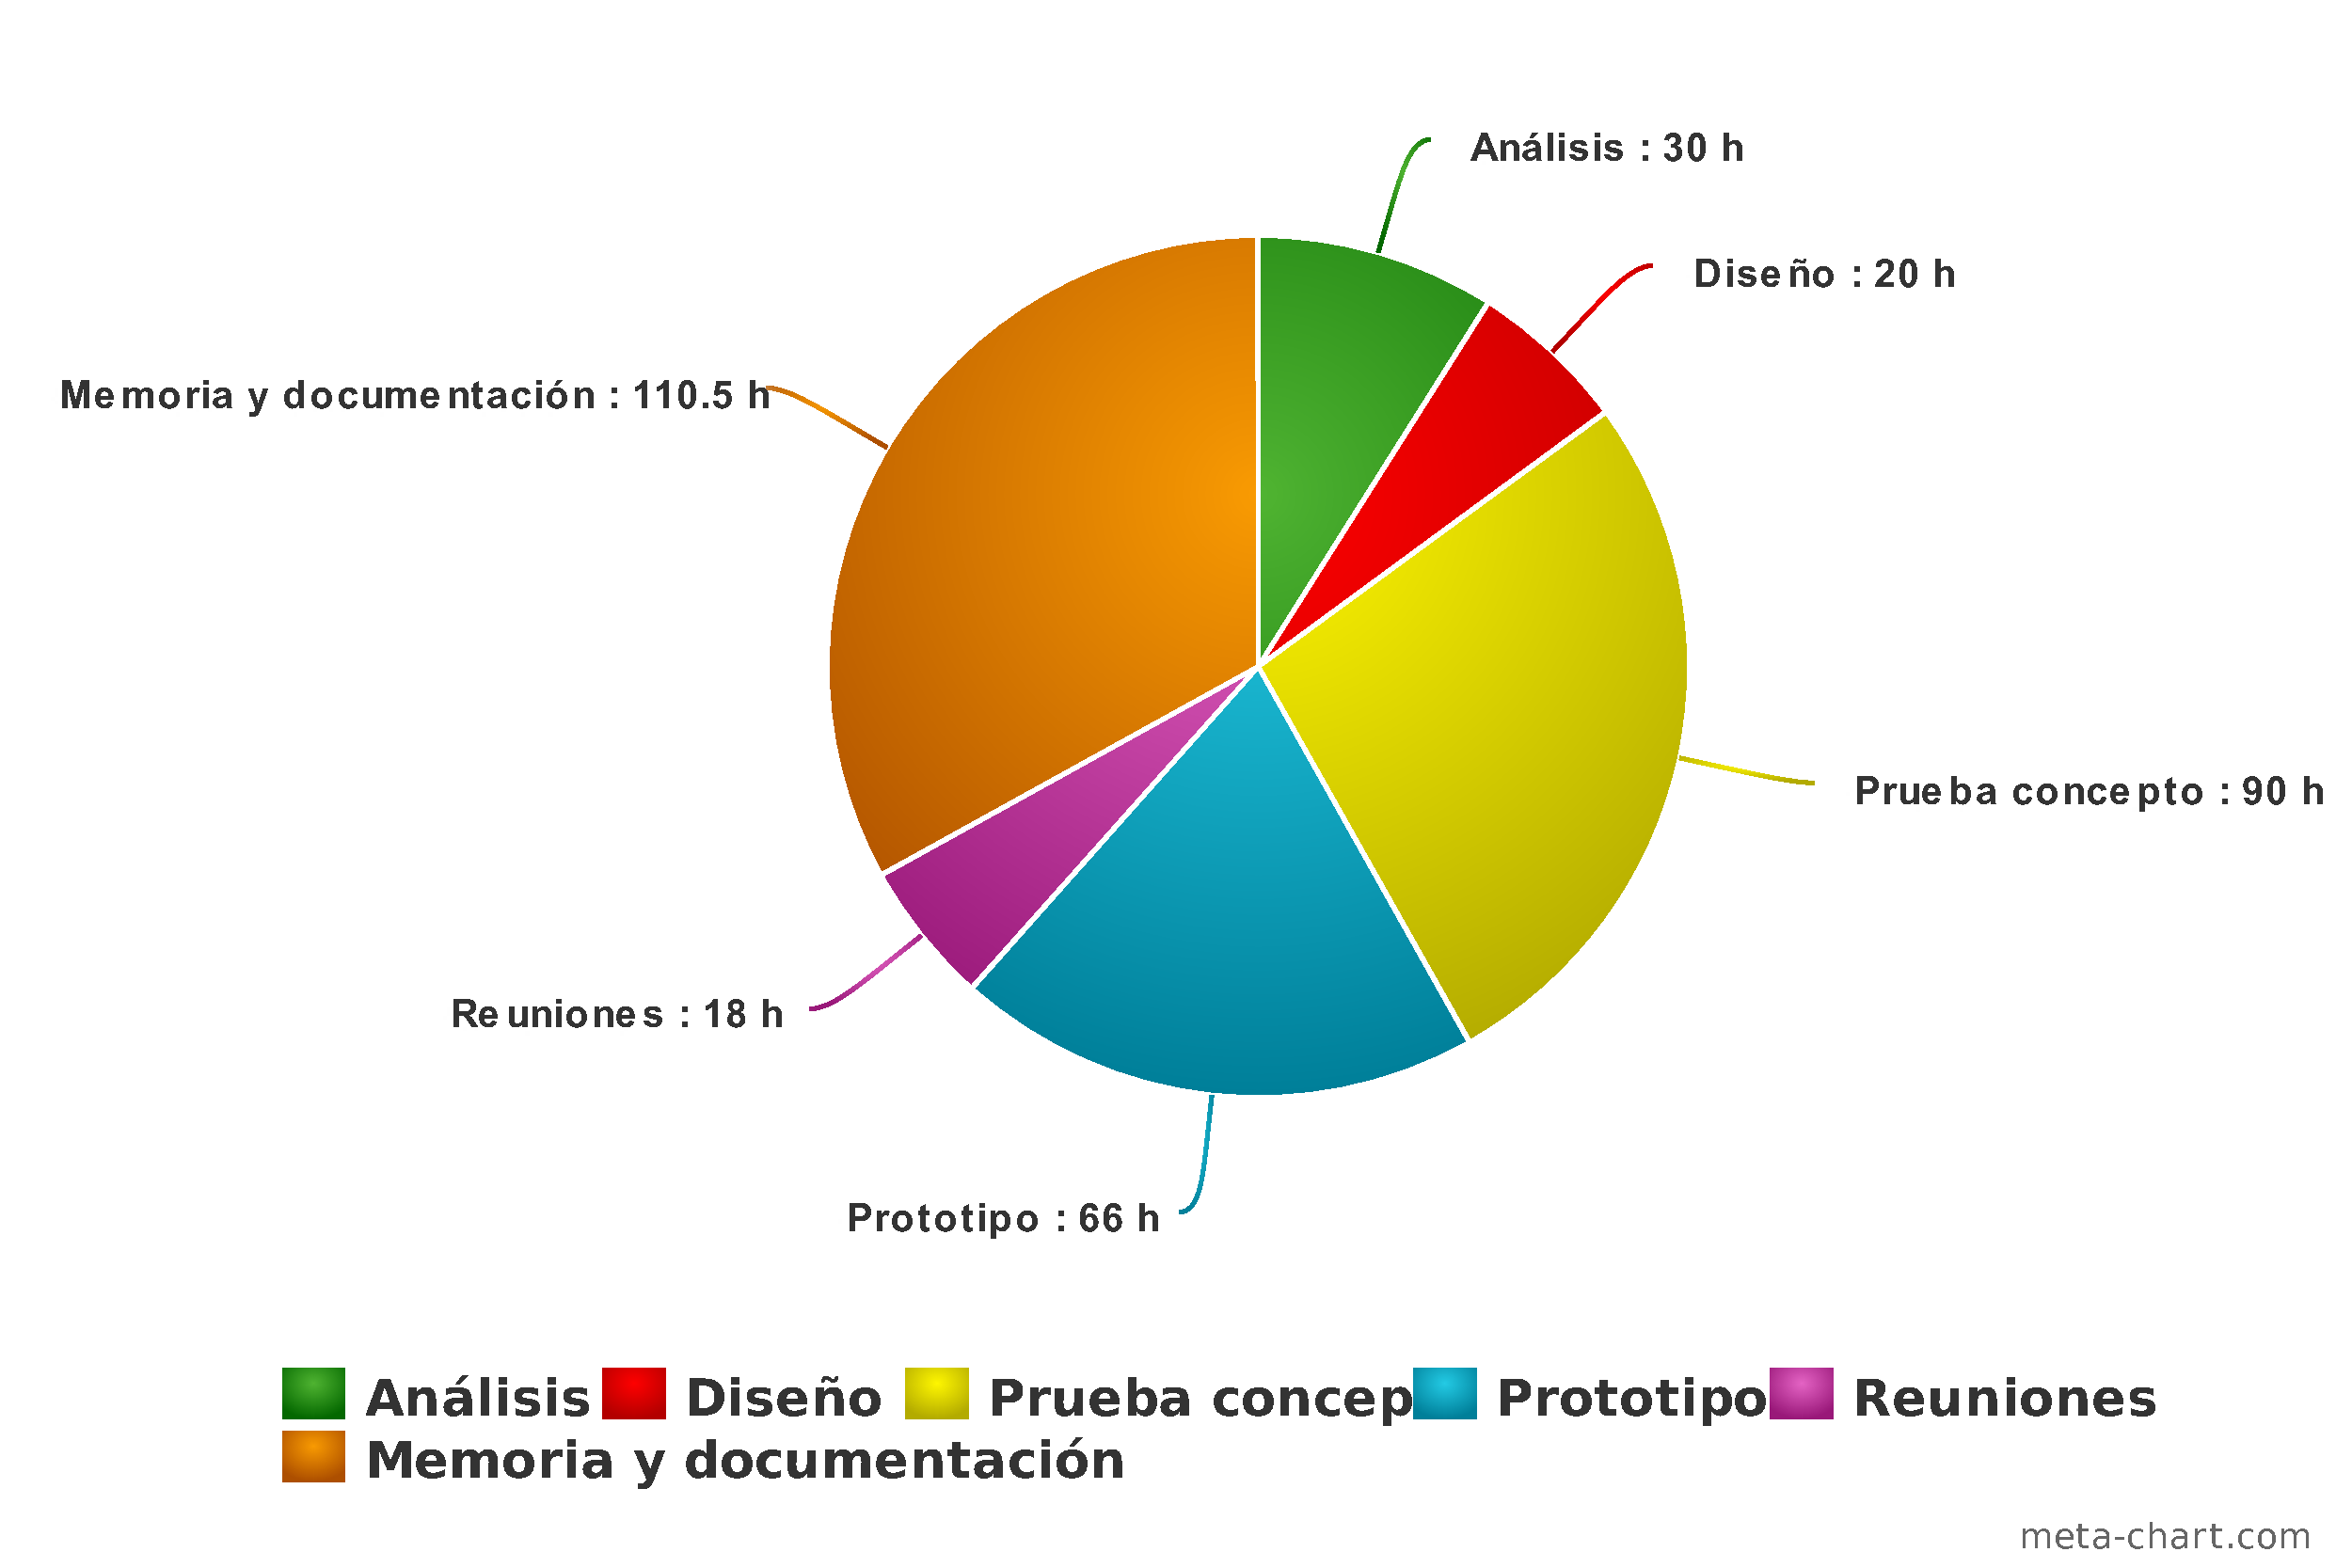
\includegraphics[width=\textwidth,height=\textheight,keepaspectratio]{Imagenes/esfuerzos}
    \caption{Horas de dedicación al proyecto.}
    \label{fig:esfuerzos}
\end{figure}


\section{Estimación del coste} \label{gestion.estimacion}

En este apartado se van a recoger los cálculos que se han llevado a cabo para calcular tanto el coste económico del \textit{TFG} como de la hora de trabajo de una persona que desarrollaría de manera comercial un proyecto como este. Para ello se ha hecho uso de la página web \textit{Calculadora Freelance} \cite{calculadorafreelance} y los resultados se pueden ver en los párrafos siguientes. 
\par 
Para calcular el coste económico del proyecto, se deben conocer a priori tanto las horas totales invertidas en el proyecto como el precio de la hora de trabajo del alumno; el resultado de la multiplicación de estos factores, sumado a otros elementos (como la gestión del proyecto, la gestión de configuraciones o el aseguramiento de la calidad), se corresponde al coste total del proyecto. Las horas invertidas en el proyecto han sido recogidas en el apartado anterior, mientras que la hora de trabajo del alumno se ha calculado a partir de los parámetros de la tabla \ref{tab:preciohora}.


\begin{table}[!h]
\centering
\bgroup
\def\arraystretch{1.3}
\begin{tabular}{l r}
\toprule
\textbf{Concepto} & \textbf{Cantidad} \\
 \midrule
 Sueldo esperado
& 
1500€ mensuales
 \\
 Días de vacaciones
& 
21 días anuales
 \\
 Días de inactividad
& 
7 días anuales
 \\
 Porcentaje reuniones, presupuestos, ventas, etc.
& 
50\%
 \\
 Gastos alquiler
& 
100€ mensuales
 \\
 Gastos en servicios (luz, móvil, etc.)
& 
50€ mensuales
 \\
 Impuesto autónomos
& 
260€ mensuales
 \\
 Otros gastos
& 
50€ mensuales
 \\
 Porcentaje beneficios
& 
20\%
\\
 \hline
 \textbf{TOTAL}
& 
\textbf{28.70€}
 \\
\bottomrule
\end{tabular}
\egroup
\caption{Precio por hora de trabajo}
\label{tab:preciohora}
\end{table}

Visto lo anterior, el coste mínimo de la hora de trabajo del alumno sería de \textbf{28.70€} y el desglose de los cálculos se puede observar en la sección \ref{d.gestion.estimacion} de los Anexos.

A continuación, en la tabla \ref{tab:costeproyecto} se recogen los diferentes componentes y tareas realizadas por el alumno junto con las horas dedicadas y el coste calculado, para conseguir el coste total del proyecto: 


\begin{table}[!h]
\centering
\bgroup
\def\arraystretch{1.3}
\begin{tabular}{l p{120pt} r}
\toprule
\textbf{Tarea/Componente} & \textbf{Horas} & \textbf{Coste (€)} \\
 \midrule
 Investigación
& 
10 horas
& 
287.00€
 \\
 Análisis
& 
20 horas
& 
574.00€
 \\
 Diseño
& 
20 horas
& 
574.00€
 \\
 Prueba de concepto
& 
80 horas
& 
2,296.00€
 \\
 Implementación prototipo
& 
63.5 horas
&
1,822.45€
 \\
 Reuniones
& 
18 horas
& 
516.60€
 \\
 Redacción Memoria
& 
110.5 horas
& 
3,171.35€
 \\
 \textbf{TOTAL Tareas/Componentes}
& 
\textbf{322 horas}
& 
\textbf{9,241.4€}
 \\
 \hline
 Gestión (G)
& 
322 h x 0.15
& 
1,269.97€
 \\
 Gestión de configuraciones (GC)
& 
322 h x 0.05
& 
462.07€
 \\
 Aseguramiento de la calidad (AC)
& 
322 h x 0.07
& 
646.90€
 \\
 \textbf{TOTAL GESTIÓN Y CALIDAD}
& 
\textbf{87 horas}
& 
\textbf{2,495.18€}
 \\
 \hline
 Transporte (T)
& 
60 viajes x 2.70€
& 
162.00€
 \\
 \textbf{TOTAL MACROS}
& 
\textit{G+GC+AC+T}
& 
\textbf{2,657.178€}
 \\
 \hline
 Amortización estaciones de trabajo
& 
(322h + 87h) x \( \frac{800}{322 h} \)
& 
985.54€
 \\
 \textbf{TOTAL}
& 
& 
\textbf{12,884.12€}
 \\
\bottomrule
\end{tabular}
\egroup
\caption{Costes económicos del proyecto}
\label{tab:costeproyecto}
\end{table}
 